\subsection{Pulssensorer}\label{sec:pulssensor}
Kroppens puls kan detekteres på en række forskellige måder, eksempelvis ved brug af en elektrisk eller optisk pulssensor. Elektriske pulssensorer måler pulsen ved hjælp af en elektrisk kontaktflade mellem sensor og person, som skabes ved hjælp af elektroder. Pulsen detekteres herved gennem forskelle i den elektriske ladning mellem elektroderne. Udfaldet af målingerne kan være afvigende, da individuelle faktorer, som en personens blod, svedniveau eller hudfedt, er en afgørende faktor for målingen. For at minimere disse udfald kræves der en god elektronisk kontakt, hvorfor præparering af huden er nødvendig.\fxnote{Kig her for at se hjertets afledninger: https://www.sundhed.dk/borger/sygdomme-a-aa/hjerte-og-blodkar/illustrationer/tegning/placering-af-ekg-elektroder/}.~\citep{PhuaLissorguesMercier2009}  \\
Optiske pulssensorer registrerer puls ved hjælp af lys. En LED udsender lys, som passerer huden og en blodåre, hvoraf en mængde af dette lys absorberes af hæmoglobin i blodet. Efterfulgt af dette opfanger en fotodiode mængden af det resterende lys. Størrelsen af dette lys er den bestemmende faktor vedrørende mængde af blod i blodåren og er heraf omvendt proportionalt. Pulssensoren udsender positive udsalg på signalet desto mere blod der registreres. Denne type sensor placeres derfor over en blodåre.~\citep{PhuaLissorguesMercier2009,SrinivasReddySrinivas2006} 

En optisk pulssensor registrerer blodomløbet i en blodåre. Blodomløbet i kroppen er kontrolleret af antallet af hjerteslag. Ét hjerteslag involverer to perioder, henholdsvis systole og diastole. I den systoliske periode kontraherer atrierne og derefter ventriklerne for dermed at pumpe blodet ud i kroppen. Efterfølgende er der en afslappende periode i hjertets muskulatur, som er den diastoliske periode. \newline
Ved at benytte en optisk sensor vil det være muligt at identificere disse perioder i hjertets cyklus. Systole kommer til udtryk med en større amplitude end diastolen, hvilket skyldes en større mængde blod under den systoliske periode. Dette fremgår desuden af \figref{fig:puls_goldenstand}, hvor et råt pulssignal er optaget med en optisk sensor.~\citep{Martini2012}
\begin{figure}[H]
	\centering
	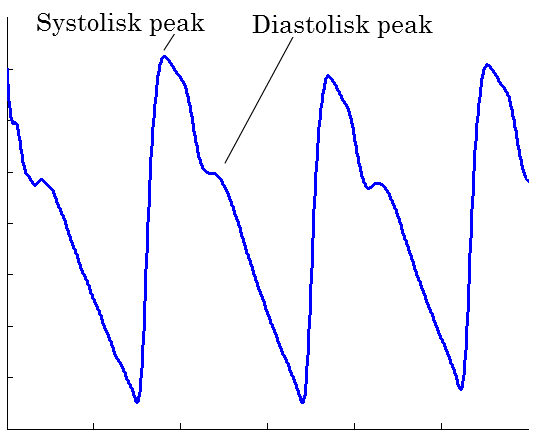
\includegraphics[scale=0.365]{figures/cDesign/puls_goldenstand.png}
	\caption{Figuren viser et pulssignal indeholdende systoliske og diastoliske peaks.~\citep{GanZahedi2011} (Modificeret)}
	\label{fig:puls_goldenstand}
\end{figure}\vspace{-0.25cm}
Én hjertecyklus og dermed ét hjerteslag involverer perioderne systole og diastole. Systole fremgår på \figref{fig:puls_goldenstand} som et peak med en stor amplitude. Det vil derfor være muligt at bestemme en persons puls ved at bestemme antallet systoliske peaks i et signal, der indenfor et givent tidsinterval kan bestemme puls som antal hjerteslag i minuttet~(BPM).